\documentclass[8pt]{article}
%%%%%%%%%%%%%%%%%%%%%%%%%%%
% Packages
%%%%%%%%%%%%%%%%%%%%%%%%%%%
\usepackage{hyperref}
\hypersetup{
  pdfauthor={Marco Arieli Herrera-Valdez},
  pdftitle={}
  pdftex,
  colorlinks=true,
  urlcolor=Bittersweet,
  linkcolor=blue,
  pdftoolbar=true,
  pdfmenubar=true,
  citecolor=Purple,
  filecolor=blue,
}
%\usepackage[spanish,es-nodecimaldot]{babel}
\usepackage{lscape}
\usepackage{setspace}
%\setstretch{1.1}
%\doublespacing
\usepackage[utf8]{inputenc}
%\usepackage[latin1]{inputenc}
%\usepackage[applemac]{inputenc}
%% Only if the base font of the document is to be different, say sans serif
% Text layout
\usepackage[T1]{fontenc}
\usepackage[scaled=0.92]{helvet}
\renewcommand*\familydefault{\sfdefault}
\usepackage{authblk}
\usepackage{graphicx}
\usepackage{python}
\usepackage{mathtools,amsfonts,amssymb,amsmath}
\usepackage[dvipsnames,svgnames,hyperref,table]{xcolor}
%\usepackage{xcolor}
\usepackage{microtype}
\usepackage{sidecap}
%\hypersetup{pdfpagemode=FullScreen}
%\usepackage[left=2.5cm,right=2.5cm,top=0cm,bottom=2cm,includehead]{geometry}
\usepackage{geometry}
\usepackage{fancyhdr}
%\pagestyle{fancyplain}
%\pagestyle{plain}
% The color packages must appear before the pdfpages package
%\usepackage{chemarr}
\usepackage{listings}
%\usepackage[normalem]{ulem}
%\usepackage[usenames,svgnames,dvipsnames]{xcolor}
%\usepackage[dvipsnames,svgnames,usenames]{xcolor}
%\usepackage{booktabs} % Top and bottom rules for table
\usepackage[font=small,labelfont=bf]{caption}
\usepackage{wrapfig}
%\usepackage{subfigure}
%\usepackage{beamerthemesplit}
\usepackage{boldline}
\usepackage{multirow}
\usepackage{multicol}
\usepackage{longtable}
\usepackage{times}
\usepackage{animate}
\usepackage{pdfpages}
\usepackage{url}
%\usepackage{multimedia}
%\usepackage{movie15}
%\usepackage{media9}
\usepackage{verbatim}
%\usepackage{pgflibraryarrows}
%\usepackage{pgflibraryshapes}
\usepackage{tikz}
%\usetikzlibrary{arrows,shapes,matrix,chains,calc,positioning}
%\usetikzlibrary{trees,mindmap}
\usepackage{ifthen}
\usepackage{animate}

% To get the envelope in the author list
\usepackage[misc]{ifsym}
%\usepackage[misc,geometry]{ifsym}

%\Letter after the name of the corresponding author

% --------------------------------------
% Bibliography
% --------------------------------------
%\usepackage[sort&compress]{natbib}
\usepackage[round,sort&compress]{natbib}
%\usepackage[numbers,sort&compress]{natbib}
%\bibliographystyle{plainnat}

% ------------------------------------------------
% Abbreviations and other commands
% ------------------------------------------------
\newcommand{\lrRound}[1]{\left(#1\right)}
\newcommand{\lrSquare}[1]{\left[#1\right]}
\newcommand{\lrSet}[1]{\left\{#1\right\}}
\newcommand{\lrAbs}[1]{\left|#1\right|}
\newcommand{\lrNorm}[1]{\left\|#1\right\|}
\newcommand{\prob}[1]{\mathbf{P}\left\{ #1\right\}}
\newcommand{\eg}{\textit{e.g.}}
\newcommand{\ie}{\textit{i.e.}}
\newcommand{\potassium}{{K$^+$}}
\newcommand{\kalium}{{K$^+$}}
\newcommand{\hydrogen}{{H$^+$}}
\newcommand{\sodium}{{Na$^+$}}
\newcommand{\natrium}{{Na$^+$}}
\newcommand{\calcium}{{Ca$^{2+}$}}
\newcommand{\chloride}{{Cl$^{-}$}}
\newcommand{\magnessium}{{Mg$^{2+}$}}
\newcommand{\concRatio}[1]{ \frac{ [{#1}]_{0} }{ [{#1}]_{1}} } 
\newcommand{\extConc}[1]{[#1]_{0}}
\newcommand{\intConc}[1]{[#1]_{1}}
\newcommand{\concNa}{[Na]}
\newcommand{\concCa}{[Ca]}
\newcommand{\concCl}{[Cl]}
\newcommand{\concK}{[K]}
\newcommand{\felis}{{{$I_{cyc}$}}}
\newcommand{\icyc}{{{$I_{cyc}$}}}
\newcommand{\Avogadro}{N_{\mathrm{A}}}
\newcommand{\absTemp}{\mathrm{T}}
\newcommand{\GasConstant}{\mathrm{R}}
\newcommand{\Faraday}{\mathrm{F}}
\newcommand{\hPlanck}{\mathrm{h}}
\newcommand{\kBoltzmann}{\mathrm{k}}
\newcommand{\kT}{\mathrm{kT}}
\newcommand{\qElementary}{\mathrm{q}}
\newcommand{\hqovertwokT}[1]{\frac{\mathrm{e_0}#1}{2\mathrm{kT}}}
\newcommand{\hqoverkT}[1]{\frac{\bathroom{e_0}#1}{\mathrm{kT}}}
\def\qovertwokT{\mathrm{\frac{e_0}{2kT}}}
\def\qoverkT{\mathrm{\frac{e_0}{kT}}}
\newcommand{\trace}[1]{{\mathrm{Tr}(#1)}}
\newcommand{\tSm}{{\mathrm{Sm}}}
\newcommand{\tSy}{{\mathrm{Sy}}}
\newcommand{\tSt}{{\mathrm{St}}}
\newcommand{\tF}{{\mathrm{F}}}
\newcommand{\tLFP}{{\mathrm{LFP}}}
\newcommand{\tATP}{{\mathrm{ATP}}}
\newcommand{\tADP}{{\mathrm{ADP}}}
\newcommand{\tCaATP}{{\mathrm{CaATP}}}
\newcommand{\tP}{{\mathrm{P}}}
\newcommand{\tNa}{{\mathrm{Na}}}
\newcommand{\tNaK}{{\mathrm{NaK}}}
\newcommand{\tNaKa}{{\mathrm{NaKa}}}
\newcommand{\tNaP}{{\mathrm{NaP}}}
\newcommand{\tNaT}{{\mathrm{NaT}}}
\newcommand{\tNaH}{{\mathrm{NaH}}}
\newcommand{\tNaCa}{{\mathrm{NaCa}}}
\newcommand{\tNaKCl}{{\mathrm{NaKCl}}}
\newcommand{\tKCl}{{\mathrm{KCl}}}
\newcommand{\tCa}{{\mathrm{Ca}}}
\newcommand{\tCl}{{\mathrm{Cl}}}
\newcommand{\tCaL}{{\mathrm{CaL}}}
\newcommand{\tE}{{\mathrm{E}}}
\newcommand{\tExtra}{{\mathrm{Extra}}}
\newcommand{\tExt}{{\mathrm{Ext}}}
\newcommand{\tI}{{\mathrm{I}}}
\newcommand{\tGlu}{{\mathrm{GluA}}}
\newcommand{\tAMPA}{{\mathrm{AMPA}}}
\newcommand{\tGABA}{{\mathrm{GABA}}}
\newcommand{\tGabaA}{{\mathrm{GabaA}}}
\newcommand{\tACh}{{\mathrm{ACh}}}
\newcommand{\tS}{{\mathrm{S}}}
\newcommand{\tSK}{{\mathrm{SK}}}
\newcommand{\tH}{{\mathrm{H}}}
\newcommand{\tK}{{\mathrm{K}}}
\newcommand{\tKaD}{{\mathrm{KaD}}}
\newcommand{\tKD}{{\mathrm{KD}}}
\newcommand{\tL}{{\mathrm{L}}}
\newcommand{\INa}{{I_\mathrm{Na}}}
\newcommand{\INaT}{{I_\mathrm{NaT}}}
\newcommand{\ICa}{{I_{\mathrm{Ca}}}}
\newcommand{\ICaL}{{I_{\mathrm{CaL}}}}
\newcommand{\IKD}{{I_{\mathrm{KD}}}}
\newcommand{\IKaD}{{I_{\mathrm{KaD}}}}
\newcommand{\IK}{{I_{\mathrm{K}}}}
\newcommand{\IAMPA}{{I_{\mathrm{AMPA}}}}
\newcommand{\INMDA}{{I_{\mathrm{NMDA}}}}
\newcommand{\IGABA}{{I_{\mathrm{GABA}}}}
\newcommand{\INaKATP}{{I_{\mathrm{NaK}}}}
\newcommand{\INaK}{{I_{\mathrm{NaK}}}}
\newcommand{\INaKa}{{I_{\mathrm{NaKa}}}}	
\newcommand{\INaCaX}{{I_{\mathrm{NaCa}}}}
\newcommand{\ILeak}{{I_{\mathrm{L}}}}
\newcommand{\stimtop}{{\textit{Top}}}
\newcommand{\stimup}{{\textit{Up}}}
\newcommand{\stimdown}{{\textit{Down}}}
\newcommand{\diffop}[2]{{\partial_{#1} #2}}
%
\newcommand{\splitPage}[4]{
\begin{minipage}{#1\textwidth}
{#2}
\end{minipage}%
\begin{minipage}{#3\textwidth}
{#4}
\end{minipage}
}

\newcommand{\figref}[1]{{Fig.~\ref{#1}}}
\newcommand{\figtworefs}[2]{{Figs.~\ref{#1}~and~\ref{#2}}}
\newcommand{\figrefs}[2]{{Figs.~\ref{#1}-\ref{#2}}}
\newcommand{\req}[1]{{Eq.~\eqref{#1}}}
\newcommand{\rtwoeqs}[2]{{Eqs.~\eqref{#1}~and~\eqref{#2}}}
\newcommand{\reqs}[2]{{Eqs.~\eqref{#1}-\eqref{#2}}}
\newcommand{\eqn}[1]{\begin{equation}#1\end{equation}}
\newcommand{\eqna}[1]{\begin{eqnarray}#1\end{eqnarray}}
\newcommand{\smalleq}[1]
{\begin{equation}{\small #1}\end{equation}}
\newcommand{\smalleqna}[1]{ 
  \begin{small} 
    \begin{eqnarray} #1 \end{eqnarray} 
  \end{small}
}
\newcommand{\tinyeqna}[1]{ 
  \begin{tiny} 
    \begin{eqnarray} #1 \end{eqnarray} 
  \end{tiny}
}
% LaTeX beamer
\newcommand{\slide}[1]{\begin{frame}#1\end{frame}}
\newcommand{\from}[1]{{\tiny From #1.}}
\newcommand{\fuente}[1]{{\tiny #1}}
\newcommand{\source}[1]{{\tiny #1}}
\newcommand{\sS}[3]{{{#1}_{#2}^{#3}}}

\newcommand{\email}{\textrm{\Letter}}
\newcommand{\corrAuthor}{\textrm{\Letter}}
\newcommand{\insp}{{National Institute of Public Health}}
\newcommand{\cisei}{{Center for Research on Infectious Diseases}}
\newcommand{\imate}{{Mathematics Institute}}
\newcommand{\unam}{{National Autonomous University of Mexico}}
\newcommand{\ua}{{University of  Arizona}}
\newcommand{\uprc}{{University of Puerto Rico in Cayey}}
\newcommand{\mbi}{{Mathematical Biosciences Institute}}
\newcommand{\osu}{{Ohio State University}}
\newcommand{\asu}{{Arizona State University}}
\newcommand{\sols}{{School of Life Sciences}}
\newcommand{\smss}{{School of Mathematical Sciences and Statistics}}
\newcommand{\mcmsc}{{Mathematical, Computational, and Modelling Sciences Center}}
\newcommand{\shesc}{School of Human Evolution and Social Change}
%
 \newcommand{\INSP}{{Instituto Nacional de Salud Pública}}
\newcommand{\CISEI}{{Centro de Investigación Sobre Enfermedades Infecciosas}}
\newcommand{\UNAM}{{Universidad Nacional Aut\'onoma de M\'exico}}
\newcommand{\IM}{{Instituto de Matem\'aticas}}
\newcommand{\IF}{{Instituto de F\'isica}}
\newcommand{\FC}{{Facultad de Ciencias}}
\newcommand{\DM}{{Departamento de Matem\'aticas}}
% \newcommand{\ua}{{Universidad de  Arizona}}
% \newcommand{\asu}{{Universidad Estatal de Arizona}}
% \newcommand{\uprc}{{Universidad de Puerto Rico en Cayey}}
% \newcommand{\mbi}{{Instituto de Biociencias Matem\UTF{00C3}\UTF{00A1}ticas}}
% \newcommand{\osu}{{Universidad Estatal de Ohio}}
% ------------------------------------------------

%%%%%%%%%%%%%%%%%%%%%%%%%%%
% Edits and reviews
%%%%%%%%%%%%%%%%%%%%%%%%%%%
\newcommand{\aquimequede}{
\vspace{1cm} \textcolor{red}
{\textbf{AQUI ME QUEDE}} \\
\vspace{1cm}}
\newcommand{\mahv}[1]{\textcolor{gray}{$^{MAHV:}$}\textcolor{orange}{#1} }




%%%%%%%%%%%%%%%%%%%%%%%%%%%
% Colored sections
%%%%%%%%%%%%%%%%%%%%%%%%%%%
\newcommand{\headcolor}[1]{\textcolor{Bittersweet}{#1}}
\newcommand{\colorsection}[1]{\section*{\headcolor{#1}}}
\newcommand{\colorsubsection}[1]{\subsection*{\headcolor{#1}}}
\newcommand{\colorparagraph}[1]{\paragraph{\headcolor{#1}}}
\definecolor{lightGray}{rgb}{0.92,0.92,0.92}


%%%%%%%%%%%%%%%%%%%%%%%%%%%
% Figure settings and inclusion/exclusion of figures from the compilation
%%%%%%%%%%%%%%%%%%%%%%%%%%%

\newcommand{\figu}[3]{
\begin{figure}{\begin{center}#3\end{center}}\caption{#1}\label{#2}\end{figure}}
\newcommand{\tablFigu}[3]{
\begin{table}\caption{#1}\label{#2}\begin{center}{#3}\end{center}\end{table}}
%
\newcommand{\smallcaption}[1]{\begin{small}\caption{{#1}}\end{small}}
%\renewcommand{\caption}[1]{\caption{\begin{small}#1\end{small}}}
\usepackage{comment}
%\excludecomment{cond}
\includecomment{cond}
\newcommand{\showfigs}[1]{}
\begin{cond}
\renewcommand{\showfigs}[1]{\begin{center}#1\end{center}}
\end{cond}

% --------------------------------------
% mahvMacros
% --------------------------------------
% For supplements
% --------------------------------------
%\newcommand{\hbAppendixPrefix}{A}
%
%\renewcommand{\thefigure}{\hbAppendixPrefix\arabic{figure}}
%\setcounter{figure}{0}
%\renewcommand{\thetable}{\hbAppendixPrefix\arabic{table}} 
%\setcounter{table}{0}
%\renewcommand{\theequation}{\hbAppendixPrefix\arabic{equation}} 
%\setcounter{equation}{0}


\newenvironment{suppFig}[4]{
  \begin{figure}[h]
    \begin{center}
      {\includegraphics[#4]{#3}} \caption{\small #1} \label{#2}
    \end{center}
  \end{figure}}

\newenvironment{tab}[3]{
\begin{table}
\begin{center}
{#3} \caption{\small #1} \label{#2}
\end{center}
\end{table}}

% Operators
\DeclareMathOperator{\Tr}{Tr}
\newcommand{\re}[1]{ {\mathfrak{Re}} \left( {#1} \right)}
\newcommand{\im}[1]{ {\mathfrak{Im}} \left( {#1} \right)}
% Transpose upperscript
\newcommand{\transp}[1]{#1^{\mathsmaller T}}

% Column vectors. Usage:
% \colvector{a\\b\\c\\d\\e}
\newcommand{\colvector}[1]{\begin{pmatrix}#1\end{pmatrix}} 

% Column vectors. Usage:
% \colvec{5}{a}{b}{c}{d}{e}
\newcount\colveccount
\newcommand*\colvec[1]{
        \global\colveccount#1
        \begin{pmatrix}
        \colvecnext
}
\def\colvecnext#1{
        #1
        \global\advance\colveccount-1
        \ifnum\colveccount>0
                \\
                \expandafter\colvecnext
        \else
                \end{pmatrix}
        \fi
}

% ----------------------------------
% Code listing 
% ----------------------------------
%\lstdefinestyle{customPython}{
%  language=Python,
%  belowcaptionskip=1\baselineskip,
%  breaklines=true,
%  %frame=L,
%  xleftmargin=\parindent,
%  showstringspaces=false,
%  basicstyle=\footnotesize\ttfamily,
%  keywordstyle=\bfseries\color{green!40!black},
%  commentstyle=\itshape\color{purple!40!black},
%  identifierstyle=\color{blue},
%  stringstyle=\color{orange},
%}

%\newcommand<>{\hover}[1]{\uncover#2{%
% \begin{tikzpicture}[remember picture,overlay]%
% \draw[fill,opacity=0.4] (current page.south west)
% rectangle (current page.north east);
% \node at (current page.center) {#1};
% \end{tikzpicture}}
%}

\usepackage[utf8]{inputenc}
\setstretch{1.3}
%
\title{Initial dynamics and general properties of case fatality ratios for Covid-19 a few weeks into the pandemic}
\author{Marco Arieli Herrera-Valdez}
\date{April 2020}
%
\begin{document}
%
\begin{flushleft}
\begin{Large}
{Initial mortality and recovery in reported cases of Covid-19 a few weeks into the pandemic}
\end{Large}\\
\smallskip
\begin{large}
Carlos Ignacio Herrera-Nolasco$^1$, Alejandro Joel Herrera-McKiernan$^2$, 
Emilio Arieli Herrera-McKiernan$^3$, Eugenia O'Reilly-Regueiro$^{4,\email}$,
Marco Arieli Herrera-Valdez$^{1,\email}$
\end{large}\\
\smallskip
$^1$ Departamento de Matemáticas, Facultad de Ciencias, Universidad Nacional Autónoma de México\\
$^2$ Escuela Primaria República de Guatemala, Secretaría de Educación Pública, México\\
$^3$ Escuela Secundaria Vicente Guerrero, Secretaría de Educación Pública, Mexico\\
$^4$ Instituto de Matemáticas, Facultad de Ciencias, Universidad Nacional Autónoma de México\\
$\email$ marcoh@ciencias.unam.mx, eugenia@im.unam.mx
\end{flushleft}

\begin{abstract} The cases, deaths, and recoveries reported by country during the initial 13 weeks of the COVID-19 pandemic are examined to estimate general properties of the propagation dynamics of disease. To get a macroscopic description of the spatio-temporal dynamics of the pandemic, we first quantified the delays between the first case reports in different countries and the delays between those first cases and the first recovery and first death in that country, respectively. We found that confirmed cases of COVID-19 epidemic had been reported from all continents but Africa within 7 days of the first confirmed case report, and cases reported also in Africa only 7 days after. We also found that the delay between the first case and the first death reported within a single country varied but had a mode at 16 days. Similarly, the delay between first  recovery and first case reported had two modes, one at 12 days, and one at 16 days. 
    We focus on the deaths by case as the most important, less unreliable indicator of the dynamics, and calculated the case fatality ratios for different countries. The case fatality ratios provide very similar estimates for the mortality rate in confirmed COVID-19 infections around the world, a reassuring feature that indicates that modeling and theoretical studies based on assumptions resting on case-fatality data may be of some utility to understand the underlying dynamics of this COVID-19 pandemic. 

\end{abstract}

\section{Introduction}
The sampling for cases and deaths from those cases in many countries are biased by the numbers of people in need for critical care that sought medical attention, by local policies triage, and by different numbers of tests \textit{per capita} administered by different governments. 

Delays between case reports and deaths... bias in the delay and under reporting...

\section{Methods and data sources} 

The data was downloaded from the repository for the 2019 Novel Coronavirus Visual Dashboard operated by the Johns Hopkins University Center for Systems Science and Engineering (JHU CSSE)  (\url{github.com/CSSEGISandData/COVID-19}). 
All calculations were performed using Python version 3.82 (\url{www.python.org}) and the modules numpy (\url{numpy.org}), matplotlib (\url{https://matplotlib.org}), and pandas (\url{pandas.pydata.org}). 
A JuPyTeR notebook with the analysis and calculations performed here can be found at (\url{scab-unam.github.io/tsam_Covid-19}).

The data considered in this analysis is between January 22 ($d_0$) and April 12, 2020 ($d_f$).

CFR ratios by age were obtained from \citep{}

%To account for the uncertainty in the delays between confirmation of cases and a deaths, the time series of deaths were divided by the time series of cases by shifting the data between 14 and 35 days, which correspond to possible delays between reports in the case of short and long time courses of disease, respectively. Notice that it is impossible for these calculations to account for under-reporting of cases.

\section{Results}


\begin{figure}[h]
    \centering
    \begin{minipage}{0.5\textwidth}
    (a)\\
    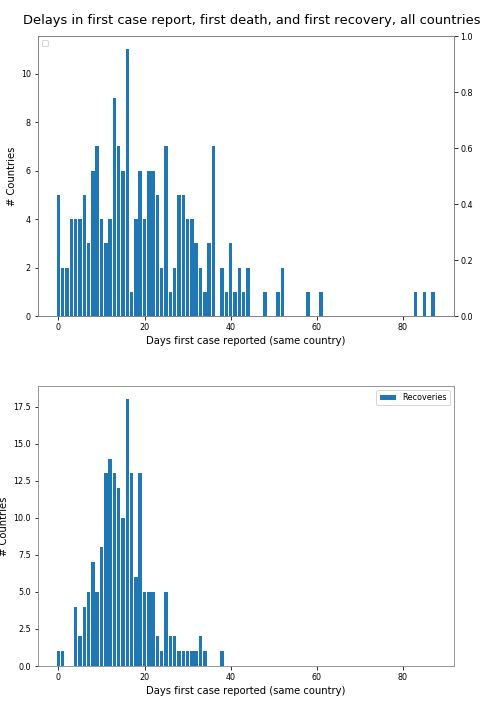
\includegraphics[width=\textwidth]{figures/tsam_Covid19_JHU_delays_AllCountries}
    \end{minipage}%
    \begin{minipage}{0.5\textwidth}
    (b)\\
    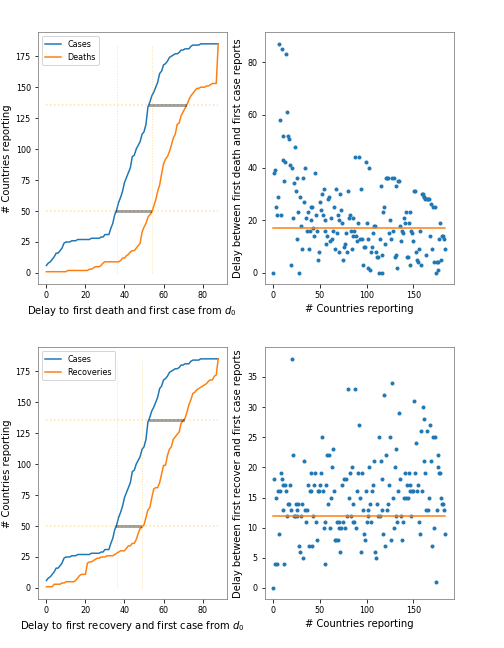
\includegraphics[width=\textwidth]{figures/tsam_Covid19_JHU_delays_caseDeaths.png}
    \end{minipage}
    \caption{From top to bottom respectively, delays (in days) between the first case reports of COVID-19 in different countries (top) relative to $d_0$, between the first death and the first case report, and  between the first recovery and the first case report 
    in each country.}
    \label{fig:caseDelays}
\end{figure}

\subsection{Delays between first case reports, first deaths, and first recoveries}

A total of 185 countries are considered in the data base, from which 175 had reported cases, up to the final report day $d_f$ 
The first countries that reported cases of Covid-19 on January 22 (day 0), 2020 were South Korea, China, Taiwan, US, Japan, and Thailand (Table~\ref{tab:delaysInReport}). Australia reported their first case 4 days later, together with Canada, on January 26, 2020. The first reports from Europe were made  on January 27, 5 days after day 0, from Germany \citep{rothe2020transmission}. The first report in the Middle East was made from the United Arab Emirates on January 29, 7 days after the first case reported.  Therefore, the COVID-19 epidemic had been reported from all continents but Africa one week after the first case was reported, and the first report from Africa arrived 23 days later from Egypt, on February 14, 2020. Of interest to the authors, Mexico reported their first case 37 days later, on February 28, 2020, together with Nigeria, New Zealand, Lithuania, Iceland, and Belarus. The last country that reported cases during the time considered for this report was Yemen , on April 11, 2020, 75 days after the first report.

Taking $d_0$ as a starting point that signaled the start of testing for Covid-19, these data indicate that confirmed  cases of COVID-19 were wide spread throughout the globe within 2 weeks of the first case, strongly suggesting that the dissemination of the SARS-CoV-2 virus among the human population occurred with a delay of approximately 2 weeks. 


The delays between the first case reported and the first death reported within a single country have a wide distribution, between 0 and 76 days. 
However, the bulk of the distribution can be found between 0 and 30 days, with a mode at 16 days. In consideration of the time course of the infection by SARS-CoV-2 reported in the literature \citep{}, the delay between death and contagion can be 21 or more days \citep{}. 

Assuming that the testing started at least one week before the date of the first case reported, the data suggest that the epidemic in those countries contributing to left portion of the histogram had started at least 3 weeks before their report. The mode at 16 days fits within the 5-7 days incubation periods reported plus the 2 weeks to develop severe symptoms. For those countries that reported their first death at the mode or after, these data suggest that the epidemic started in those countries at least one week before their first case reported.

The delays between the first recovery and the first case reported within a single country are distributed between 0 and 38 days. However, for most countries this delay is between 0 and 27 days approximately, with two clear modes at 12 and 16 days.  

\subsection{Case fatality ratios}

\begin{figure}[h]
    \centering
    \begin{minipage}{0.5\textwidth}
    (a)\\
    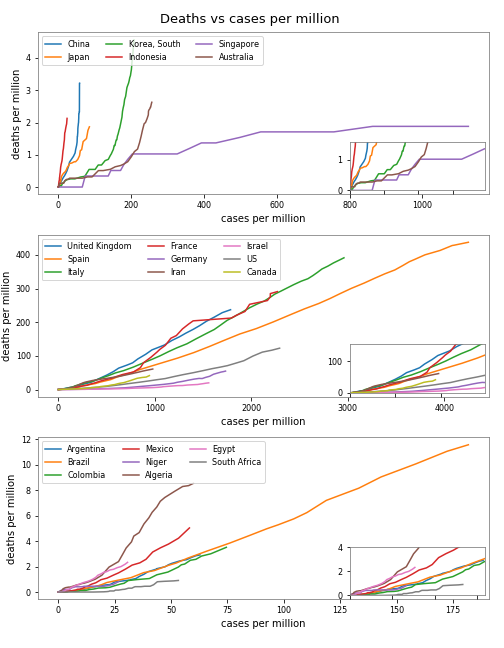
\includegraphics[width=\textwidth]{figures/tsam_Covid19_JHU_cases-deaths_x1000000_JHU.png}
    \end{minipage}%
    \begin{minipage}{0.5\textwidth}
    (b)\\
    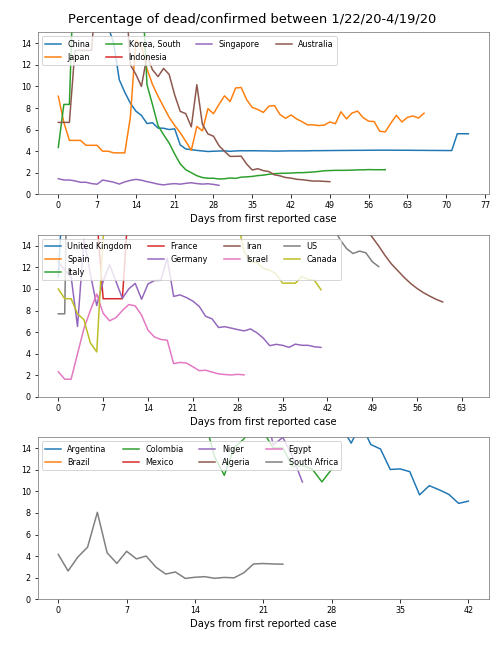
\includegraphics[width=\textwidth]{figures/tsam_Covid19_JHU_cfr_fromFirstLocalCase.png}
    \end{minipage}
    \caption{(a) Deaths vs cases (per million people) in different countries. (b) CFRs relative to the first local report.}
    \label{fig:casesDeaths1000}
\end{figure}

\subsubsection{Case fatality ratios are lower when calculated by province}

\begin{figure}[h]
    \centering
    \begin{minipage}{0.6\textwidth}
    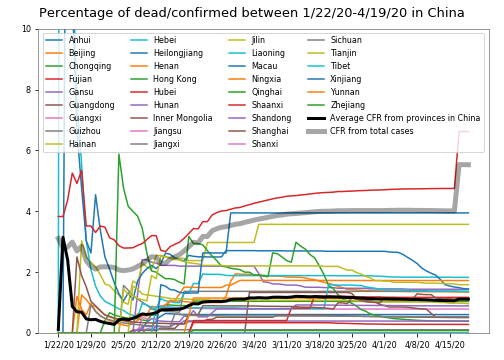
\includegraphics[width=\textwidth]{figures/tsam_Covid19_JHU_cfr_ProvincesChina_fromFirstLocalReport}
    \end{minipage}%
    \begin{minipage}{0.4\textwidth}
    \caption{CFRs by province in China (top). The average CFR from the provinces is shown in black. The CFR from the total cases is shown as a gray thick line.}
    \label{fig:cfrsProvinces}
    \end{minipage}
\end{figure}

\subsubsection{CFRs increase with age, mostly for adults after 30 years old}

\begin{figure}[h]
    \centering
    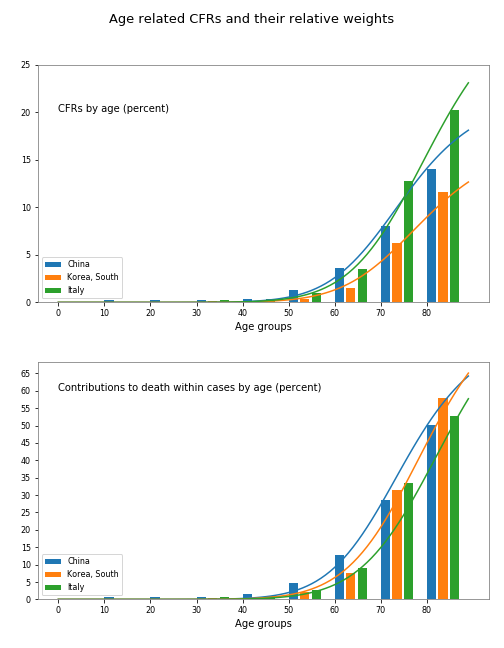
\includegraphics[width=\textwidth]{figures/tsam_Covid19_JHU_cfr+propDeathCases_ByAge_China+SKorea+Italy_OneFigure.png}
    \caption{CFRs age in South Korea (top), Italy (middle), and China (bottom).}
    \label{fig:cfrsAge}
\end{figure}

\subsubsection{Estimates of the time dependence of the CFR by age for South Korea, Italy, and China}

\begin{figure}[h]
    \centering
    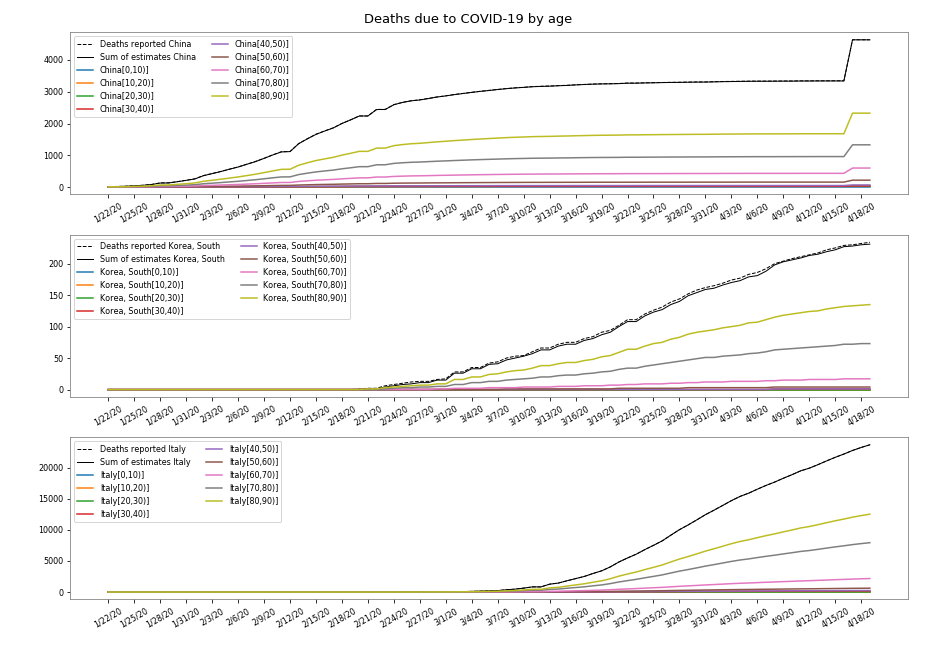
\includegraphics[width=\textwidth]{figures/tsam_Covid19_JHU_cfr+propDeathCasesByAgeTS.png}
    \caption{Time series estimations of CFRs age in South Korea (top), Italy (middle), and China (bottom).}
    \label{fig:cfrsAge}
\end{figure}



\subsubsection{Estimates for Mexico using the age-CFRs from three different countries reveal similar patterns}

\begin{figure}[h]
    \centering
    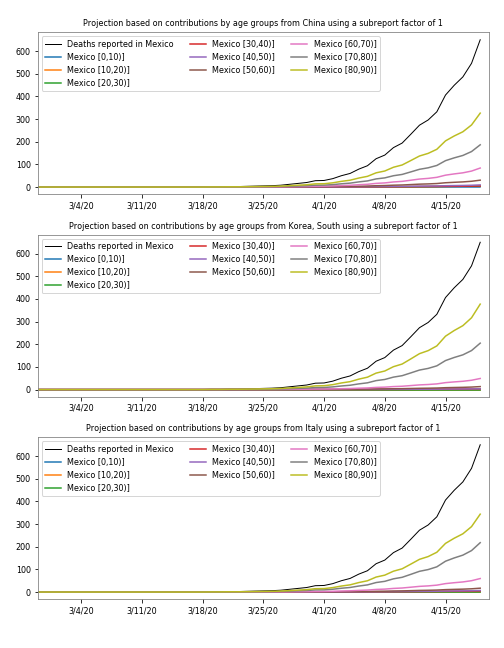
\includegraphics[width=\textwidth]{figures/tsam_Covid19_JHU_cfr+propDeathCasesByAgeTS_EstimatesMexico_subReportFactor1.png}
    \caption{The weights of the CFRs by age from South Korea (top), Italy (middle), and China (bottom) were used to estimate the contributions to death cases in Mexico.}
    \label{fig:cfrsAge}
\end{figure}


\section{Discussion}



\paragraph{Contributions:} CIH-N,EO-R, and MAH-V  wrote the manuscript; AJH-M, EAH-M, MAH-M, collected data spread sheets, examined maps, websites, performed the exploratory analysis and created the initial plots that gave support to the claims made in this report. CIH-N, MAH-V,and EO-R discussed the results, and formalised the analysis; and MAH-V wrote python scripts and the JuPyTeR notebooks and setup the website for supplementary materials to this report. 

\paragraph{Acknowledgments:} Funding was provided for MAHV by PAPIME-UNAM grant PE-114919.

\newpage
\section{Appendix}
% !TEX root = COVID-19_cfr.tex
\begin{table}[h]
\caption{Delays to the first reports relative to the first COVID-19 case in January 22, 2020 ($d_0$).}\label{tab:delaysInReport} 
\begin{longtable}{p{0.3\textwidth} c c c}
\hline %
Country & First case from $d_0$, & to first death & to first recovery \\
\line \\
China & 1/22/20 (0)  & 1/22/20 (0)  & 1/22/20 (0) \\
US & 1/22/20 (0)  & 2/29/20 (38)  & 2/9/20 (18) \\
Thailand & 1/22/20 (0)  & 3/1/20 (39)  & 1/26/20 (4) \\
Taiwan* & 1/22/20 (0)  & 2/16/20 (25)  & 2/6/20 (15) \\
Japan & 1/22/20 (0)  & 2/13/20 (22)  & 1/26/20 (4) \\
Korea, South & 1/22/20 (0)  & 2/20/20 (29)  & 2/7/20 (16) \\
\hline 
Vietnam & 1/23/20 (1)  & 4/11/20 (79)  & 2/1/20 (9) \\
Singapore & 1/23/20 (1)  & 3/21/20 (58)  & 2/8/20 (16) \\
\hline 
France & 1/24/20 (2)  & 2/15/20 (22)  & 2/12/20 (19) \\
\hline 
Nepal & 1/25/20 (3)  & 4/11/20 (77)  & 2/12/20 (18) \\
Malaysia & 1/25/20 (3)  & 3/17/20 (52)  & 2/7/20 (13) \\
\hline 
Canada & 1/26/20 (4)  & 3/9/20 (43)  & 2/12/20 (17) \\
Australia & 1/26/20 (4)  & 3/1/20 (35)  & 1/30/20 (4) \\
\hline 
Germany & 1/27/20 (5)  & 3/9/20 (42)  & 2/13/20 (17) \\
Cambodia & 1/27/20 (5)  & 4/11/20 (75)  & 2/12/20 (16) \\
Sri Lanka & 1/27/20 (5)  & 3/28/20 (61)  & 2/8/20 (12) \\
\hline 
Finland & 1/29/20 (7)  & 3/21/20 (52)  & 2/12/20 (14) \\
United Arab Emirates & 1/29/20 (7)  & 3/20/20 (51)  & 2/12/20 (14) \\
\hline 
India & 1/30/20 (8)  & 3/11/20 (41)  & 2/16/20 (17) \\
Philippines & 1/30/20 (8)  & 2/2/20 (3)  & 2/12/20 (13) \\
\hline 
Sweden & 1/31/20 (9)  & 3/11/20 (40)  & 3/9/20 (38) \\
Italy & 1/31/20 (9)  & 2/21/20 (21)  & 2/22/20 (22) \\
United Kingdom & 1/31/20 (9)  & 3/5/20 (34)  & 2/12/20 (12) \\
Russia & 1/31/20 (9)  & 3/19/20 (48)  & 2/12/20 (12) \\
\hline 
Spain & 2/1/20 (10)  & 3/3/20 (31)  & 2/15/20 (14) \\
\hline 
Belgium & 2/4/20 (13)  & 3/11/20 (36)  & 2/17/20 (13) \\
\hline 
Diamond Princess & 2/7/20 (16)  & 2/20/20 (13)  & 2/19/20 (12) \\
\hline 
Egypt & 2/14/20 (23)  & 3/8/20 (23)  & 2/28/20 (14) \\
\hline 
Iran & 2/19/20 (28)  & 2/19/20 (0)  & 2/26/20 (7) \\
\hline 
Israel & 2/21/20 (30)  & 3/21/20 (29)  & 2/27/20 (6) \\
Lebanon & 2/21/20 (30)  & 3/10/20 (18)  & 3/4/20 (12) \\
\hline 
Iraq & 2/24/20 (33)  & 3/4/20 (9)  & 3/9/20 (14) \\
Oman & 2/24/20 (33)  & 3/31/20 (36)  & 2/29/20 (5) \\
Afghanistan & 2/24/20 (33)  & 3/22/20 (27)  & 3/16/20 (21) \\
Kuwait & 2/24/20 (33)  & 4/4/20 (40)  & 3/8/20 (13) \\
Bahrain & 2/24/20 (33)  & 3/16/20 (21)  & 3/6/20 (11) \\
\hline 
Austria & 2/25/20 (34)  & 3/12/20 (16)  & 3/9/20 (13) \\
Croatia & 2/25/20 (34)  & 3/19/20 (23)  & 3/13/20 (17) \\
Switzerland & 2/25/20 (34)  & 3/5/20 (9)  & 3/3/20 (7) \\
Algeria & 2/25/20 (34)  & 3/12/20 (16)  & 3/12/20 (16) \\
\hline 
Brazil & 2/26/20 (35)  & 3/17/20 (20)  & 3/16/20 (19) \\
North Macedonia & 2/26/20 (35)  & 3/22/20 (25)  & 3/13/20 (16) \\
Romania & 2/26/20 (35)  & 3/22/20 (25)  & 3/4/20 (7) \\
Norway & 2/26/20 (35)  & 3/14/20 (17)  & 3/9/20 (12) \\
Greece & 2/26/20 (35)  & 3/11/20 (14)  & 3/14/20 (17) \\
Georgia & 2/26/20 (35)  & 4/4/20 (38)  & 3/16/20 (19) \\
Pakistan & 2/26/20 (35)  & 3/19/20 (22)  & 3/8/20 (11) \\
\hline 
Denmark & 2/27/20 (36)  & 3/14/20 (16)  & 3/6/20 (8) \\
San Marino & 2/27/20 (36)  & 3/3/20 (5)  & 3/14/20 (16) \\
Netherlands & 2/27/20 (36)  & 3/6/20 (8)  & 3/14/20 (16) \\
Estonia & 2/27/20 (36)  & 3/25/20 (27)  & 3/15/20 (17) \\
\hline 
Nigeria & 2/28/20 (37)  & 3/23/20 (24)  & 3/18/20 (19) \\
New Zealand & 2/28/20 (37)  & 3/29/20 (30)  & 3/24/20 (25) \\
Lithuania & 2/28/20 (37)  & 3/21/20 (22)  & 3/15/20 (16) \\
Belarus & 2/28/20 (37)  & 3/31/20 (32)  & 3/9/20 (10) \\
Mexico & 2/28/20 (37)  & 3/19/20 (20)  & 3/3/20 (4) \\
Iceland & 2/28/20 (37)  & 3/15/20 (16)  & 3/10/20 (11) \\
\hline 
Ireland & 2/29/20 (38)  & 3/11/20 (11)  & 3/17/20 (17) \\
Luxembourg & 2/29/20 (38)  & 3/14/20 (14)  & 3/22/20 (22) \\
Qatar & 2/29/20 (38)  & 3/28/20 (28)  & 3/14/20 (14) \\
Monaco & 2/29/20 (38)  & 3/29/20 (29)  & 3/22/20 (22) \\
\hline 
Azerbaijan & 3/1/20 (39)  & 3/13/20 (12)  & 3/11/20 (10) \\
Czechia & 3/1/20 (39)  & 3/22/20 (21)  & 3/16/20 (15) \\
Ecuador & 3/1/20 (39)  & 3/14/20 (13)  & 3/21/20 (20) \\
Dominican Republic & 3/1/20 (39)  & 3/17/20 (16)  & 3/24/20 (23) \\
Armenia & 3/1/20 (39)  & 3/26/20 (25)  & 3/17/20 (16) \\
\hline 
Indonesia & 3/2/20 (40)  & 3/11/20 (9)  & 3/10/20 (8) \\
Latvia & 3/2/20 (40)  & 4/3/20 (32)  & 3/10/20 (8) \\
Portugal & 3/2/20 (40)  & 3/17/20 (15)  & 3/13/20 (11) \\
Saudi Arabia & 3/2/20 (40)  & 3/24/20 (22)  & 3/10/20 (8) \\
Morocco & 3/2/20 (40)  & 3/10/20 (8)  & 3/13/20 (11) \\
Andorra & 3/2/20 (40)  & 3/22/20 (20)  & 3/12/20 (10) \\
Senegal & 3/2/20 (40)  & 4/1/20 (30)  & 3/8/20 (6) \\
\hline 
Jordan & 3/3/20 (41)  & 3/27/20 (24)  & 3/13/20 (10) \\
Chile & 3/3/20 (41)  & 3/22/20 (19)  & 3/20/20 (17) \\
Argentina & 3/3/20 (41)  & 3/8/20 (5)  & 3/14/20 (11) \\
Ukraine & 3/3/20 (41)  & 3/13/20 (10)  & 3/21/20 (18) \\
\hline 
Hungary & 3/4/20 (42)  & 3/15/20 (11)  & 3/14/20 (10) \\
Tunisia & 3/4/20 (42)  & 3/19/20 (15)  & 3/22/20 (18) \\
Poland & 3/4/20 (42)  & 3/12/20 (8)  & 3/16/20 (12) \\
Liechtenstein & 3/4/20 (42)  & 4/4/20 (31)  & 4/6/20 (33) \\
\hline 
West Bank and Gaza & 3/5/20 (43)  & 3/26/20 (21)  & 3/20/20 (15) \\
South Africa & 3/5/20 (43)  & 3/27/20 (22)  & 3/24/20 (19) \\
Bosnia and Herzegovina & 3/5/20 (43)  & 3/21/20 (16)  & 3/17/20 (12) \\
Slovenia & 3/5/20 (43)  & 3/14/20 (9)  & 3/25/20 (20) \\
\hline 
Peru & 3/6/20 (44)  & 3/20/20 (14)  & 3/17/20 (11) \\
Togo & 3/6/20 (44)  & 3/27/20 (21)  & 3/20/20 (14) \\
Colombia & 3/6/20 (44)  & 3/22/20 (16)  & 3/17/20 (11) \\
Holy See & 3/6/20 (44)  & 4/11/20 (36)  & 4/8/20 (33) \\
Serbia & 3/6/20 (44)  & 3/20/20 (14)  & 3/16/20 (10) \\
Slovakia & 3/6/20 (44)  & 3/18/20 (12)  & 3/22/20 (16) \\
Cameroon & 3/6/20 (44)  & 3/25/20 (19)  & 3/25/20 (19) \\
Bhutan & 3/6/20 (44)  & 4/11/20 (36)  & 4/2/20 (27) \\
Costa Rica & 3/6/20 (44)  & 3/19/20 (13)  & 3/21/20 (15) \\
\hline 
Malta & 3/7/20 (45)  & 4/8/20 (32)  & 3/13/20 (6) \\
\hline 
Paraguay & 3/8/20 (46)  & 3/21/20 (13)  & 3/27/20 (19) \\
Bulgaria & 3/8/20 (46)  & 3/11/20 (3)  & 3/21/20 (13) \\
Moldova & 3/8/20 (46)  & 3/18/20 (10)  & 3/17/20 (9) \\
Bangladesh & 3/8/20 (46)  & 3/18/20 (10)  & 3/16/20 (8) \\
Maldives & 3/8/20 (46)  & 4/11/20 (34)  & 3/24/20 (16) \\
\hline 
Brunei & 3/9/20 (47)  & 3/28/20 (19)  & 3/20/20 (11) \\
Cyprus & 3/9/20 (47)  & 3/22/20 (13)  & 3/22/20 (13) \\
Albania & 3/9/20 (47)  & 3/11/20 (2)  & 3/21/20 (12) \\
\hline 
Mongolia & 3/10/20 (48)  & 4/11/20 (32)  & 3/30/20 (20) \\
Panama & 3/10/20 (48)  & 3/11/20 (1)  & 3/24/20 (14) \\
Burkina Faso & 3/10/20 (48)  & 3/18/20 (8)  & 3/21/20 (11) \\
\hline 
Congo (Kinshasa) & 3/11/20 (49)  & 3/21/20 (10)  & 3/27/20 (16) \\
Honduras & 3/11/20 (49)  & 3/26/20 (15)  & 3/28/20 (17) \\
Bolivia & 3/11/20 (49)  & 3/29/20 (18)  & 4/1/20 (21) \\
Cote d'Ivoire & 3/11/20 (49)  & 3/29/20 (18)  & 3/17/20 (6) \\
Jamaica & 3/11/20 (49)  & 3/19/20 (8)  & 3/16/20 (5) \\
Turkey & 3/11/20 (49)  & 3/17/20 (6)  & 3/25/20 (14) \\
\hline 
Cuba & 3/12/20 (50)  & 3/18/20 (6)  & 3/24/20 (12) \\
Guyana & 3/12/20 (50)  & 3/12/20 (0)  & 4/6/20 (25) \\
\hline 
Kenya & 3/13/20 (51)  & 3/26/20 (13)  & 3/25/20 (12) \\
Guinea & 3/13/20 (51)  & 4/11/20 (29)  & 4/3/20 (21) \\
Sudan & 3/13/20 (51)  & 3/13/20 (0)  & 3/31/20 (18) \\
Kazakhstan & 3/13/20 (51)  & 3/20/20 (7)  & 3/26/20 (13) \\
Ethiopia & 3/13/20 (51)  & 4/5/20 (23)  & 3/22/20 (9) \\
Antigua and Barbuda & 3/13/20 (51)  & 4/7/20 (25)  & 4/11/20 (29) \\
\hline 
Trinidad and Tobago & 3/14/20 (52)  & 3/25/20 (11)  & 3/21/20 (7) \\
Rwanda & 3/14/20 (52)  & 4/11/20 (28)  & 4/5/20 (22) \\
Saint Lucia & 3/14/20 (52)  & 4/11/20 (28)  & 3/27/20 (13) \\
Saint Vincent and the Grenadines & 3/14/20 (52)  & 4/11/20 (28)  & 3/28/20 (14) \\
Uruguay & 3/14/20 (52)  & 3/29/20 (15)  & 3/31/20 (17) \\
Suriname & 3/14/20 (52)  & 4/3/20 (20)  & 4/8/20 (25) \\
Venezuela & 3/14/20 (52)  & 3/27/20 (13)  & 3/22/20 (8) \\
Seychelles & 3/14/20 (52)  & 4/11/20 (28)  & 4/11/20 (28) \\
Mauritania & 3/14/20 (52)  & 3/30/20 (16)  & 3/29/20 (15) \\
Namibia & 3/14/20 (52)  & 4/11/20 (28)  & 3/24/20 (10) \\
Gabon & 3/14/20 (52)  & 3/20/20 (6)  & 4/3/20 (20) \\
Ghana & 3/14/20 (52)  & 3/21/20 (7)  & 3/26/20 (12) \\
Eswatini & 3/14/20 (52)  & 4/11/20 (28)  & 4/6/20 (23) \\
Guatemala & 3/14/20 (52)  & 3/16/20 (2)  & 3/25/20 (11) \\
\hline 
Equatorial Guinea & 3/15/20 (53)  & 4/11/20 (27)  & 3/31/20 (16) \\
Central African Republic & 3/15/20 (53)  & 4/11/20 (27)  & 4/11/20 (27) \\
Congo (Brazzaville) & 3/15/20 (53)  & 4/2/20 (18)  & 4/2/20 (18) \\
Uzbekistan & 3/15/20 (53)  & 3/27/20 (12)  & 3/27/20 (12) \\
\hline 
Bahamas & 3/16/20 (54)  & 4/1/20 (16)  & 3/24/20 (8) \\
Tanzania & 3/16/20 (54)  & 3/31/20 (15)  & 3/27/20 (11) \\
Benin & 3/16/20 (54)  & 4/6/20 (21)  & 3/31/20 (15) \\
Liberia & 3/16/20 (54)  & 4/4/20 (19)  & 4/4/20 (19) \\
Somalia & 3/16/20 (54)  & 4/8/20 (23)  & 3/31/20 (15) \\
\hline 
Montenegro & 3/17/20 (55)  & 3/23/20 (6)  & 4/3/20 (17) \\
Gambia & 3/17/20 (55)  & 3/23/20 (6)  & 4/1/20 (15) \\
Barbados & 3/17/20 (55)  & 4/5/20 (19)  & 4/5/20 (19) \\
\hline 
Djibouti & 3/18/20 (56)  & 4/10/20 (23)  & 4/3/20 (16) \\
Mauritius & 3/18/20 (56)  & 3/21/20 (3)  & 4/4/20 (17) \\
Kyrgyzstan & 3/18/20 (56)  & 4/3/20 (16)  & 3/30/20 (12) \\
Zambia & 3/18/20 (56)  & 4/2/20 (15)  & 4/3/20 (16) \\
\hline 
El Salvador & 3/19/20 (57)  & 3/31/20 (12)  & 4/4/20 (16) \\
Fiji & 3/19/20 (57)  & 4/11/20 (23)  & 4/11/20 (23) \\
Chad & 3/19/20 (57)  & 4/11/20 (23)  & 4/7/20 (19) \\
Nicaragua & 3/19/20 (57)  & 3/27/20 (8)  & 4/11/20 (23) \\
\hline 
Niger & 3/20/20 (58)  & 3/25/20 (5)  & 4/5/20 (16) \\
Cabo Verde & 3/20/20 (58)  & 3/24/20 (4)  & 4/6/20 (17) \\
Angola & 3/20/20 (58)  & 3/29/20 (9)  & 3/31/20 (11) \\
Haiti & 3/20/20 (58)  & 4/5/20 (16)  & 3/29/20 (9) \\
Zimbabwe & 3/20/20 (58)  & 3/23/20 (3)  & 4/11/20 (22) \\
Madagascar & 3/20/20 (58)  & 4/11/20 (22)  & 4/5/20 (16) \\
Papua New Guinea & 3/20/20 (58)  & 4/11/20 (22)  & 4/11/20 (22) \\
\hline 
Uganda & 3/21/20 (59)  & 4/11/20 (21)  & 4/11/20 (21) \\
Eritrea & 3/21/20 (59)  & 4/11/20 (21)  & 4/11/20 (21) \\
\hline 
Timor-Leste & 3/22/20 (60)  & 4/11/20 (20)  & 4/10/20 (19) \\
Syria & 3/22/20 (60)  & 3/29/20 (7)  & 4/4/20 (13) \\
Grenada & 3/22/20 (60)  & 4/11/20 (20)  & 4/11/20 (20) \\
Mozambique & 3/22/20 (60)  & 4/11/20 (20)  & 4/4/20 (13) \\
Dominica & 3/22/20 (60)  & 4/11/20 (20)  & 4/6/20 (15) \\
\hline 
Belize & 3/23/20 (61)  & 4/6/20 (14)  & 4/11/20 (19) \\
\hline 
Laos & 3/24/20 (62)  & 4/11/20 (18)  & 4/11/20 (18) \\
Libya & 3/24/20 (62)  & 4/2/20 (9)  & 3/31/20 (7) \\
\hline 
Saint Kitts and Nevis & 3/25/20 (63)  & 4/11/20 (17)  & 4/11/20 (17) \\
Mali & 3/25/20 (63)  & 3/29/20 (4)  & 4/4/20 (10) \\
Guinea-Bissau & 3/25/20 (63)  & 4/11/20 (17)  & 4/11/20 (17) \\
\hline 
Kosovo & 3/26/20 (64)  & 3/26/20 (0)  & 3/27/20 (1) \\
\hline 
Burma & 3/27/20 (65)  & 3/31/20 (4)  & 4/9/20 (13) \\
\hline 
MS Zaandam & 3/28/20 (66)  & 4/1/20 (4)  & 4/11/20 (14) \\
\hline 
Botswana & 3/30/20 (68)  & 3/31/20 (1)  & 4/11/20 (12) \\
\hline 
Burundi & 3/31/20 (69)  & 4/11/20 (11)  & 4/11/20 (11) \\
Sierra Leone & 3/31/20 (69)  & 4/11/20 (11)  & 4/11/20 (11) \\
\hline 
Malawi & 4/2/20 (71)  & 4/7/20 (5)  & 4/11/20 (9) \\
\hline 
Western Sahara & 4/5/20 (74)  & 4/11/20 (6)  & 4/11/20 (6) \\
South Sudan & 4/5/20 (74)  & 4/11/20 (6)  & 4/11/20 (6) \\
\hline 
Sao Tome and Principe & 4/6/20 (75)  & 4/11/20 (5)  & 4/11/20 (5) \\
\hline 
Yemen & 4/10/20 (79)  & 4/11/20 (1)  & 4/11/20 (1) \\
\hline
\end{longtable}
\end{table}


\bibliographystyle{plainnat}
\bibliography{COVID-19.bib}
\end{document}
